\chapter{Results}\label{cha:results}

%Guideline
    % introduction
    % LED PCB and spi captures >> 
    %     challenges only in communication
    %     improvements
    % Scheduling 
    %     TAble with challenges and results
    %     final comments and improvements
    % SOES
    %     Wireshark and twincat screenshots
    %     Challenges breaking the infinite loops and the CPs
        
This chapter starts where the previous chapter left for each of the functional modules, having in mind that the results for the 
temperature are mixed with those of SOES, as the data that is being transferred is now only generated by the sensors. Some photos
and screenshots are presented as well. Challenges, their solving and further improvements are also commented along the chapter.


\section{PCB, SPI and LED control}

In Fig.~\ref{fig:pcb_final} the final PCB prototype can be seen. It is worth mentioning that one issue
emerged
related to the physical requirements of the temperature sensors. 
According to the library integration process commented in Sect.~\ref{sec:temperature}, 
during the first month a rather simplistic approach was coded to have access to the temperature values, the sensors in this approach
used an 
external power source. In contrast, the final sensors were cabled in such a way that they rely on parasite-powered circuitry.
Additionally, the final library that was included made use of the UART peripheral in a full duplex mode, which means that two independent 
pins were explicitly needed, namely RX and TX. That also differed from the first approach's configuration mode. Given this differences, 
only one available GPIO pin with no extra pull-up transistor in the PCB side, was not appropriate to test correctly the 
new one-wire setup. Nonetheless, arrangements were carried out to use the UART RX/TX pins available in the JTAG connector and add external resistors. 
This approach was merely for testing and will be corrected in any further development out of the scope of this Research Project.

\begin{figure}
  \centering
  \subfigure[PCB unmounted]{\label{subfig:pcb_final1}{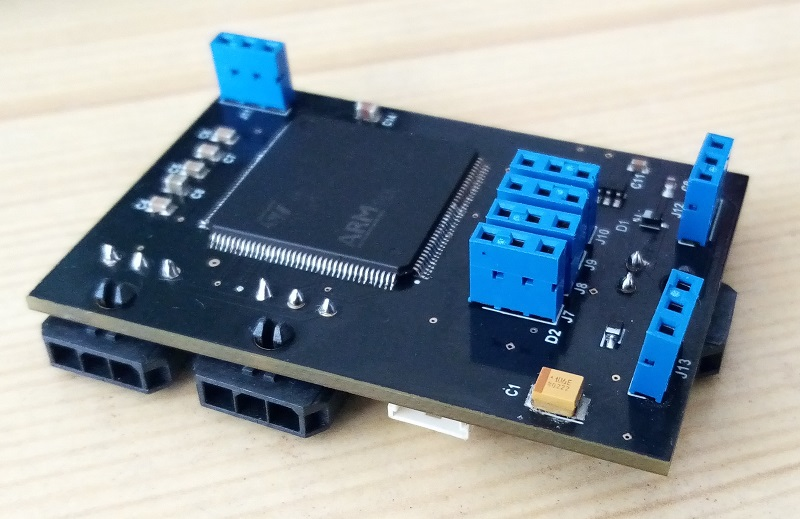
\includegraphics[width=0.42\textwidth]{imgs/res-pcb01.jpg}}}\hfill
  \subfigure[PCB mounted]{\label{subfig:pcb_final2}{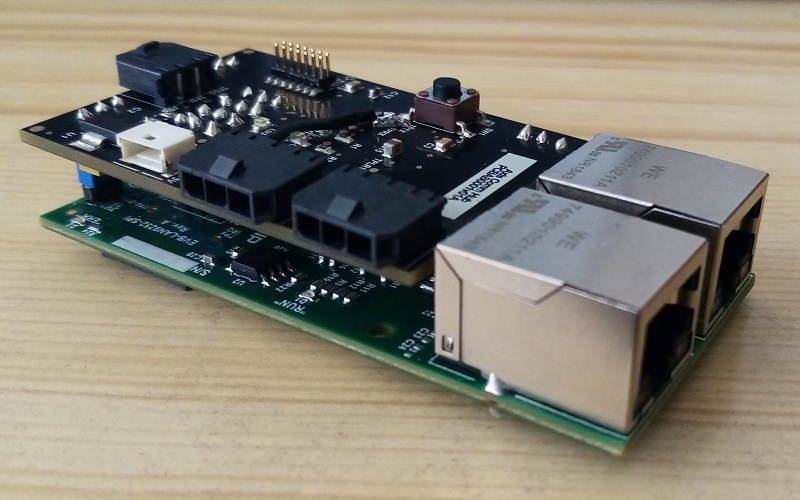
\includegraphics[width=0.42\textwidth]{imgs/res-pcb02.jpg}}}
  \caption{Manufactured PCB.}
  \label{fig:pcb_final}
\end{figure}

The Process Data Interface (PDI) took into consideration the minimal data rate 
calculated for unsigned integers of 16-bit long that would be interpreted
by the Master. This information is summarized in Table~\ref{tbl:minimal_speed}. 

\begin{tuhhtable}
  \begin{tabular}[tp]{L{.18\textwidth}C{.35\textwidth}C{.3\textwidth}}
    \THc{1}{c}{Data} &  \THc{1}{c}{Considerations}&  \THc{1}{c}{Size} \\
    \abovebodyrule
      Temperature       & 15 sensors   &  \SI{30}{\byte}     \\\TRc
      System     & Status, events, errors and parameters data chunk    & \SI{8}{\byte}     \\
      Master               & Commands data chunk& \SI{8}{\byte}     \\\TRc
      IMU            & Acceleration, Magnetometer and Gyroscope for 3 Axis & \SI{36}{\byte}    \\
      BISS-C                 & Data chunk      & \SI{12}{\byte}    \\
    \belowbodyrule
    Total                 &       & \SI{94}{\byte} $\sim$ \SI{128}{\byte}    \\\TRc
    Data rate @ \SI{10}{\milli\second}                 &       & \SI{12.8}{\kilo\byte\per\second}$=$\SI{0.1}{\mega\bit\per\second}   \\
  \end{tabular}
  \caption{Data chunks considered for calculating a minimal data rate at the required refresh rate of the device. }
  \label{tbl:minimal_speed}
\end{tuhhtable}

Another issue that is good to remark, is the noisy communication that emerged at SPI higher speeds. Generally, the monitoring of SPI
signals was very frequently, since the possibility of a fault increased after any new modification, and those needed to be 
traced back to their origin, being sometimes the Host MCU or the LAN9252 chip. Nevertheless, hooking up to the SPI bus introduced another
fault source that was not identified until the communication speeds and their quality were generally characterized. This is, if the GPIOs were 
adjusted to be visualized through a logic analyzer or oscilloscope the communication with LAN9252 was not possible. Hence, 
in order to keep a reliable test environment, it was decided to decrease the SPI data rate without affecting the minimal 
settings 
previously mentioned in Table~\ref{tbl:minimal_speed}. Note that that higher data rate configuration does not imply higher data transmission, as 
the library introduces an almost constant software delay due to the processing of the stack functions, 
namely between \SIrange{2.7}{2.9}{\micro\second}; which starts to be significant as the interface speed goes up. 
The observations regarding this issue are presented in Table~\ref{tbl:spi_speeds}, where symbols imply how good or bad was the communication
between the MCU host and LAN9252, and the visibility through an oscilloscope or digital analyzer. As to the noisy channels at 
high speeds, two screenshots can be seen in Fig.~\ref{fig:signal_noisy}. 

This overall signal integrity problem is rather common within hardware design, therefore, longer times are needed to 
fulfill the requirements
of an optimized hardware when it comes to sensitive data signals. The mentioned working line itself is very broad and 
an introduction for how grounding affects the signal integrity can be consulted in ~\cite{pcb_design_grounding}.%add the reference of pcb desginf for high frequency


%Configuration  GPIO characteristic Speed   LAN9252 stability Logic analizer 
\begin{tuhhtable}
    \begin{tabular}[tp]{C{.14\textwidth}L{.23\textwidth}C{.23\textwidth}C{.23\textwidth}}
      \THc{1}{c}{Config} &  \THc{1}{c}{GPIO setup}& \THc{1}{c}{LAN9252 comm}& \THc{1}{c}{Signal visibility} \\
      \abovebodyrule
        1       & PU: SS\newline NPU/NPD:\newline SCK/MOSI/MISO   & @\SI{10}{\mega\bit\per\second} \tblBad  & \tblGood     \\\TRc
        2       & PU: SS\newline NPU/NPD:\newline SCK/MOSI/MISO   & @\SI{20}{\mega\bit\per\second} \tblBad  & \tblFair\\
        3       & PU: SS\newline NPU/NPD:\newline SCK/MOSI/MISO   & @\SI{40}{\mega\bit\per\second} \tblBad  & \tblBad  \\\TRc
        4       & NPU/NPD:\newline SCK/SS/MOSI/MISO        & @\SI{2.5}{\mega\bit\per\second} \tblGood  & \tblFair  \\\
        5       & NPU/NPD:\newline SCK/SS/MOSI/MISO        & @\SI{20}{\mega\bit\per\second} \tblFair  & \tblBad  \\\TRc
        6       & NPU/NPD:\newline SCK/SS/MOSI/MISO        & @\SI{40}{\mega\bit\per\second} \tblFair  & \tblBad  \\
        Current         & NPU/NPD: \newline SCK/SS/MOSI/MISO       & \SI{10}{\mega\bit\per\second} \tblGood  & \tblBad  \\\TRc
      \belowbodyrule
    \end{tabular}
    \caption{SPI GPIO configurations affected the communication performance with LAN9252. PU stands for pull-up, whereas NPD, no pull-up nor pull-down. }
    \label{tbl:spi_speeds}
\end{tuhhtable}

\begin{figure}[tp]
    \centering
    \subfigure[Non Pulled-up signal]{\label{subfig:signal_weak}{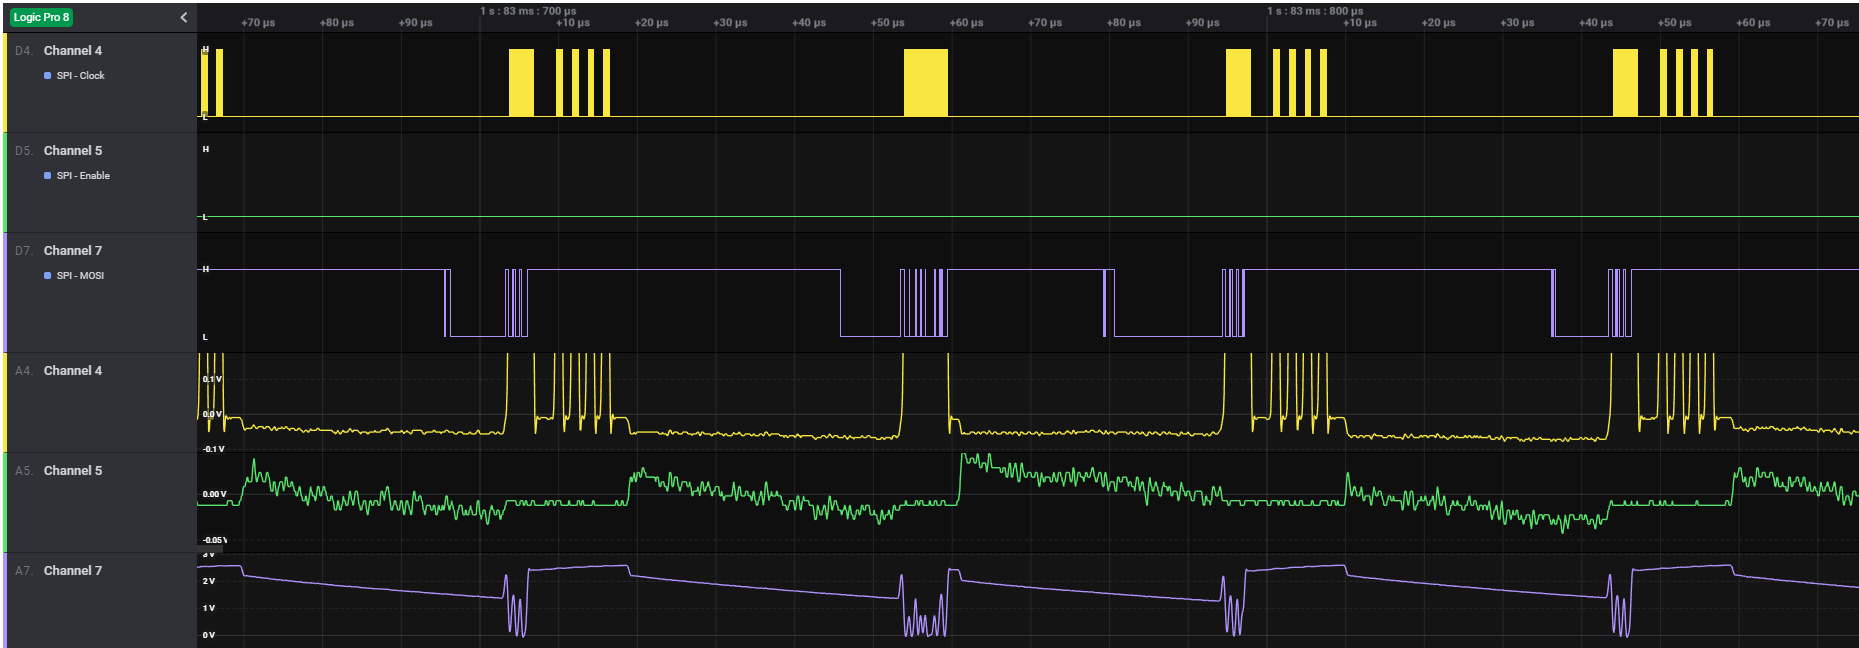
\includegraphics[width=\textwidth]{imgs/result-signalweak.png}}} \\
    \subfigure[Spikes at higher data rates]{\label{subfig:signal_noisy}{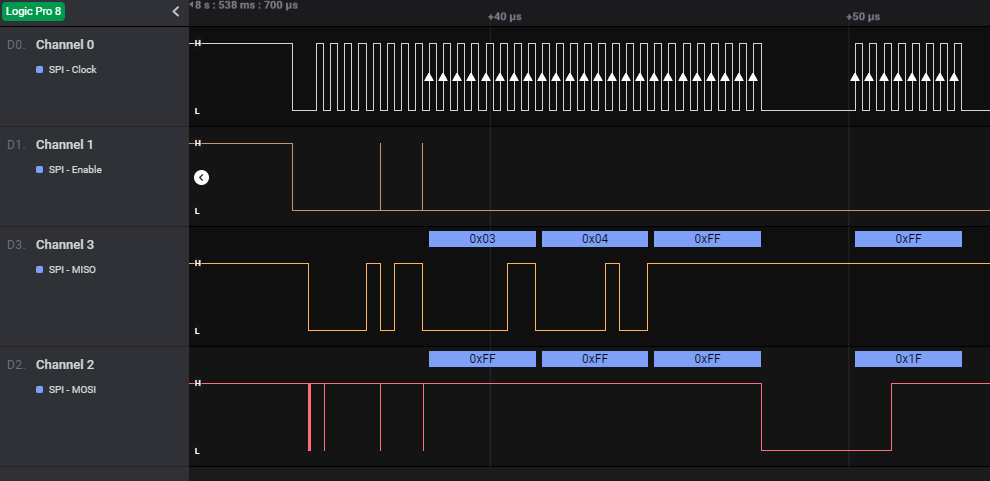
\includegraphics[width=\textwidth]{imgs/result-signalnoisy.png}}}
    \caption{Issues with SPI bus. In ~\ref{subfig:signal_weak} the green signal corresponds to SS pin and demands a pull-up resistor to proper visualization, while LAN9252 demands open-drain pin for correct communication.
            Whereas in ~\ref{subfig:signal_noisy} channels \numlist{1;2;3} show spikes that emerged frequently at speeds higher than \SI{5}{\mega\bit\per\second}, leading to an incorrect recognition of the clock (CLK) signal.}
    \label{fig:signal_noisy}
\end{figure}


With reference to the LED results, besides the challenge that personally represented the library adaptation and the usage of the DMA 
peripheral, the functionality was stable.

An open point which did not represent an obstacle for the project, but keeps the door open for further improvement is 
the possibility of using more than one channel per PWM generator. The reason why this was not implemented lies with 
the time required for testing. The straightforward option is to use one DMA channel and one PWM Channel per ring, 
for the MCU host contains two DMA peripherals, each with 8 streams and each stream in turn with 8 channels---technical
specifications can be seen in ~\cite{stm32f446_data}; 
therefore, it did not represent any problem. 
Nonetheless, it could be argued that only one PWM generator could control up to four Led Rings, as long as each PWM channel is updated through
an individual DMA channel, this way the hardware would be used more efficiently. The MCU should only have ready each memory buffer 
to start the transmission of the serial data. This approach would apparently imply larger space, but if the color data 
is taken 
out from an unique buffer that is updated on-the-fly for the next LED interface, the efficiency, at least regarding usage of HW, will be better. 
Consequently, this could also lead to use two DMA streams at the same time for a total of eight rings with only two PWM generators 
and two DMA streams. 

Anyhow, the before mentioned approach needs expertise with DMA peripheral and formal evaluation of the benchmarks related to 
the utilization
of the processor and memory footprint moreover, the optimization of this LED control is not part of the scope of this project, and 
better use of this peripheral is apparently exploited in other applications such as graphics rendering---see application in ~\cite{stm32_dmaapp}---or 
transferring of
memory chunks at way faster speeds. The latter could be though interesting, since the LAN9252 counts with a Quad-SPI interface.
%https://auto.siili.com/blog/optimizing-rendering-performance-on-stm32-using-dma2d
%Add reference to the Direct memory access DMA




\section{DSMs and RTOS integration}\label{sec:scheduling_results}

%Guidelines
% introduction
% --------------------
%     Mention the scheduling apporach of RTOS
        
%         List of proposed threads and description of them (only proposal)
%         Priority based, fixed and not based on Execution times
%            >> Time proposed for each one, mention that it is also configurable. 
%           SPI speed calculation?
%         This is a Table
     
% ---------------------This is in results-----------------------------------
%     Problems in the implementation 
%         Priority of each task + timer priority
%             Solutions + Task manager
%          Present the final table of threads
%         explains events its problems with timers, etc    
%             Solutions
%     List of resources that might demand mutex
%             List of general variables
%         Regardinf the synchronization: How the OS prevents from problems?
%             solutions
%           Future improvement (3 items for OS debugging)

As introduced during the implementation description, Sect.~\ref{sec:scheduling_intro}, this part will comment a bit further the results
of the usage of FreeRTOS to schedule and synchronize the execution of the DSMs, such that a deterministic behavior 
could be reached. Similar to the previous section, some issues and comments about it are presented along the
way.
\subsection{Final scheduling and synchronization}
To start with, in the Table~\ref{tbl:threads_final} the current list of threads can be seen. Important to point out is the necessity 
to define carefully priorities besides the previously given \emph{desired} release times. In the same table an 
OS-defined thread is included that was crucial for the current SW structure, namely \emph{osTimer Daemon Task}. 

\begin{tuhhtable}
    \begin{tabular}[hb]{L{.3\textwidth}C{.3\textwidth}C{.3\textwidth}}
      \THc{1}{c}{Thread} &  \THc{1}{c}{Priority}&  \THc{1}{c}{Release period} \\
      \abovebodyrule
        User Task Manager       & osPriorityHigh    & Event driven     \\\TRc
        osTimer Daemon Task     & osPriorityHigh    & Event driven     \\
        Event Handler SDM               & osPriorityAboveNormal& Event driven     \\\TRc
        SOES APP SDM            & osPriorityAboveNormal& \SIrange{5}{10}{\milli\second}     \\
        LED SDM                 & osPriorityNormal      & \SI{33}{\milli\second}    \\\TRc
        ECAT SDM*               & osPriorityNormal      & \SI{100}{\milli\second}     \\
        Temperature SDM         & osPriorityNormal      & \SI{1000}{\milli\second}     \\\TRc
      \belowbodyrule
    \end{tabular}
    \caption{Final priorities' arrangement for main threads. \emph{*ECAT SDM 
        is mainly event driven, nevertheless, in the connected state it has a periodic update}}
    \label{tbl:threads_final}
\end{tuhhtable}

Regarding the \emph{User Task Manager}, its implementation was meaningful because of the suspension/termination of threads was taken place
within the synchronization of ECAT and SOES DSMs---recall the synchronization signals in the DSM in Sect.~\ref{sec:statemachines}. 
For instance, due to the way the library is coded, every time there is a communication breakdown, SOES goes into an infinite loop 
as it is polling continuously ESC state registers instead of using and IRQ pin---review SM-Synchronous in Appendix~\ref{sec:synch_managers}---. 
Other sources of this infinite loops that demands forcing a thread to stop are the physical connection problems, such as the ESC power-off, 
cable disconnection, power source drop, etc. 
Given these scenarios, clearly a solution with timeout control was tried out but the low level timers (HW peripherals) induced problems
as it is of high caution mixing hardware interrupts when running an OS.
Therefore, the Task Management events are sent with help of callback functions from osTimers (Timers implemented by the OS). 
As to the latter, they are really managed by the so-called osTimer Daemon Task and are fully configurable. However, a few characteristics need to be taken 
into account as the Daemon runs as hidden Task for the user, in addition, if this Task is not correctly set the callbacks can be lost 
as the Damon tries to interrupt a higher priority task. Some parameters to configure are callback stack depth, queue length and priority. 
More information regarding this topic can be found in \emph{Timer Management} section of ~\cite{cmsis_doc}.

Coming back to the infinite loop issue, once the timers are set and can correctly interrupt, if one task is within an infinite loop, keeping its own 
state machine from continue and consequently others, then a fault is emerged. Then the osTimer creates an event and suspend or restart the faulty threads.
However, this is actually something that the Event Handler should take care of, or any other thread, since the OS-defined functions
related to thread management cannot be executed from ISR ---not even software interruptions. Furthermore, the suspension or termination of
threads need to be handled with care, since if a thread is suspended or terminated right after a higher priority task preempts the callback
function---imagine the Event Handler SDM being of higher priority than SOES App SDM---as soon as the higher priority task finishes, the callback 
function would be executed but as the OS would try to
go back to the thread where it was originally called, and this has been put out of the execution queue, it would result in an OS hard fault.

Therefore, using a simple user-defined Task Manager thread that is constantly waiting for event flags or periodically updating their states, 
makes possible to manipulate threads, and therefore it has been the current solution to avoid some problems. However, 
less complicated approaches are being taken
into account for further generalization, since deleting and creating tasks might have stability problems regarding the fragmentation
of the heap. Sometimes, hard faults may appear and would be very hard to identify which memory overflow might have caused it.

Just as the previous example, hard faults---not surprisingly---are to be avoided, but doing this efficiently demands rather \emph{good strategy}.
What is more, this situation could repeat in other conditions, even due to implementation of the OS. For example, there are even 
OS-functions that are explicitly described as being compatible with execution from ISRs, though they might have no effect, as it was the 
case for Event Flags---even ensuring
their respective volatile definitions; or in the case of waiting states within a DSM. The last-mentioned can also lead to hard fault, 
since the execution of an unique Task 
that ends up calling apparently endless osDelay functions is considered as faulty condition by the OS.

\begin{tuhhtable}
  \begin{tabular}[ht]{L{.25\textwidth}L{.5\textwidth}}
    \THc{1}{c}{DSM Event} &  \THc{1}{c}{Main use} \\
    \abovebodyrule
      SYS\_EVENT    & Events and errors sent to the Event Handler DSM\\\TRc
      LED\_EVENT    & Internal LED DSM events\\
      TSENS\_EVENT  & Internal Temperature DSM events\\\TRc
      ECAT\_EVENT   &  Synchronization between ECAT DSM and SOES APP\\
      TASKM\_EVENT  & Thread management/update request from any DSM\\\TRc
    \belowbodyrule
  \end{tabular}
  \caption{Events between DSMs are implemented over \emph{Event Flag Signals} managed by the OS.}
  \label{tbl:events_sms}
\end{tuhhtable}

In relation to the mentioned synchronization events, the \emph{OS Event Flags Signals} feature was used. This is basically 32-bit long 
data shared between threads and managed by the OS, that can be related to suspension and resume of threads according to the bits (flags)
that are set or clear with \emph{OS Wait} functions. Some details could be not as clear as they should be, since working conditions
vary among OS layers, this is for example, the FreeRTOS defines the signals as 32-bit unsigned integer with the 31st bit reserved for internal
error flag; nonetheless, on top of it the CMSIS v2 defines in turn the same signal as the same integer but only 24 bits available. 
If 
the application works with any flag bit between the 24th and the 30th bit, the final OS layer returns no error but does not notify any
thread. A list of the main signals used for synchronization between DSM is presented in Table~\ref{tbl:events_sms}, whereas a list of the events
and errors so far implemented in the Event Handler DSM's logic is showed in Table~\ref{tbl:events_errors}. However, a complete list of events and
errors can be seen in the header code within Appendix~\ref{appx:code}.

\begin{tuhhtable}
  \begin{tabular}[bp]{L{.3\textwidth}L{.4\textwidth}}
    \THc{1}{c}{ACB Event} &  \THc{1}{c}{ACB Error} \\
    \abovebodyrule
      EV\_TEMP\_DSM\_INIT       &  ERR\_TEMP\_DSM\_FAULT     \\\TRc
      EV\_LED\_DSM\_INIT     &   ERR\_TEMP\_SENS\_OVERHEAT   \\
      EV\_ECAT\_DSM\_INIT               &ERR\_TEMP\_SENS\_LOST*  \\\TRc
      EV\_ECAT\_CMD\_ACK            &ERR\_LED\_DSM\_FAULT \\
      EV\_ECAT\_APP\_OP                 &   ERR\_ECAT\_DSM\_FAULT    \\\TRc
      EV\_ECAT\_APP\_INIT              & ERR\_ECAT\_CMD\_FAULT*      \\
      EV\_ECAT\_CMD\_ACK         & ERR\_ECAT\_CMD\_SOFTFAULT*      \\\TRc
        &ERR\_ECAT\_COMM\_LOST\\
        &ERR\_SYS\_UNKNOWN\\\TRc
    \belowbodyrule
  \end{tabular}
  \caption{DSM's events and errors considered by Event Handler DSM. \emph{*Currently being implemented.}}
  \label{tbl:events_errors}
\end{tuhhtable}

\subsection{Further development}
Finally, there are two topics open for future, first one has to do with shared memory, while the second is about optimization of the
scheduling approach. Regarding the former, so far no complication has appeared in the rather non-critical data being transmitted, namely
the buffer that both the Temperature and the SOES App update. Currently, an approach an easy approach that can be implemented is using
again the events to notify the SOES APP whenever the Temperature App has updated its buffer. Other is using the MUTEX feature implemented
in the OS. Both approaches are planned. Going back to the mentioned topics, the latter could be at this stage difficult, as it needs
the precise execution time of each Task to be known. Without it is not possible 
to think about optimizing the utilization or the OS configuration in a more detailed manner -if even required-. 
For instance, in the future calculation 
of the \emph{Utilization} factor will be helpful for optimizing scheduling, but it could be also needed in more practical design cases, 
e.g., 
while considering heat sinks for processors within enclosed devices. Therefore, the following is a list of proposed 
activities that could take place in future stages out of scope of the current Research Project. 

\begin{description}
\item[Execution Time estimation per task] Each task can be isolated by software. Then, by adding a piece of code to toggle a free GPIO 
      at the end of the thread, a signal can be traced with a fair digital analyzer. Omitting the rather small HAL 
      overhead added with the GPIO control, an estimation of the execution time can be achieved.
\item[Live thread tracing]  A trace debugging like SEGGER SystemView, see ~\cite{rtos_segger},%**reference to fastbitlab** 
    can be used to debug freeRTOS applications running on ARM Cortex Mx based Microcontroller such as STM32Fx. 
    With this tool it could be possible to have at runtime a trace of the thread allocations, knowing in consequence the duration 
    of the threads. 
\item[Optimization of threads] By knowing the Worst Case Execution Time (WCET) of each thread an optimization of the utilization could be carried out 
    by using different OS-native features to improve the scheduling, as long as the application demands it.
\end{description}

\section{SOES library integration}

The results presented in this section implies the correct functionality of the temperature functional block.
% Understand the variations between Little/Big Endian within buses. That the library is based on polling by one by one the unique FIFO register of the ESC, such that the PDOs can be written and read in the PD RAM, as it was thought that a direct access to the RAM would permit the User Address Space of the MCU to be extended and the access then would be transparent for manipulating the data,  and that the SM would permit only the safe access from the Master device to read/write the same address space. It could be then understood that there is a significant delay that van be even measure, that in some papers is determined as "Stack Delay" which in this case *Reference the paper of the design of the communication/delay analysis*.
% The advantages of reducing it through the implementation of the SQI or the HSI interface -which at the end does not have that much purpose since for achieving less delays the FPGA or ASIC maybe implemented-. The question, is it still sensible to develop EtherCAT devices with this approach or should it be switched completely to the FPGA and ASIC approach. An analysis considering costs and other things could be then carried out. ***
% **Making available the Szstem Interrupt Controller without polling would also increase the performance of the application, this can be aimed in next versions where physically the the pins are connected to the Host MCU.
% **A brief analysis of the bandwidht achieved as the bandwidth necessarz to make sensible a change of PDI would make sensce, since the HBI****reference to internet or anz specification of HBI*** is mainly foucsed to Board-To-Board connections or communication between ASICS, hence  4Gbps per pin die-to-die connectivity with low latency may not be needed at all *https://www.synopsys.com/designware-ip/interface-ip/die-to-die.html**.
% **Important to mention is the HBI only helps exchanging process data, so it could be implemented for applications where data chunks are needed to be transmitted at high bandwidth since it is a direct fifo access to the ESC's SRAM.
% **Here should be also commented the problems by reading and writing, mainly writting due to the noisy medium (cabling).
In the Fig.~\ref{fig:ecat_wireshark} the transition from safe-operation (SAFEOP) to operation state (OP) of the EtherCAT device is shown. 
The operation state can only be reached when the Object Dictionary has been correctly matched between the Master and the device
through the SMs, a synchronization mode has been correctly configured and the AL registers can be correctly read and written 
by both devices. The protocol makes use of DLL commands to broadcast state change requests to the slaves, afterwards it broadcasts 
a read command. Each device connected will react and update its corresponding AL state register. 

\begin{figure}[h]
  \centering
  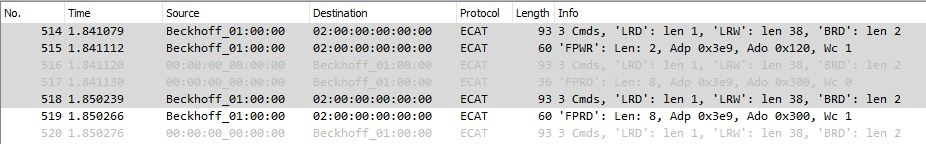
\includegraphics[width=\textwidth]{imgs/result-wireshark-preop-op1.JPG}
  \caption{Transaction of data frames between Master and Slave during a state change request.}
  \label{fig:ecat_wireshark}
\end{figure}

In addition, it is important to 
recall that the working counter at the end of the data structure that points out whether a device in the network has processed 
the data frame or not, review the frame structure in Appendix~\ref{sec:ecat_protocol}. Having the frame in mind, it is possible to 
recognize all its parts, as the the communication trace was monitored with Wireshark. Hence the detailed interaction between parties 
through the updated data frames is clearly seen in Fig.~\ref{fig:ecat_wireshark2}.


\begin{figure}[ht]
  \centering
  \subfigure[BRD command to read current AL state register]{\label{subfig:cmd1}{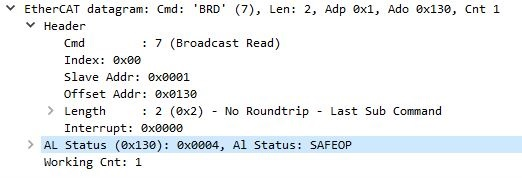
\includegraphics[width=0.7\textwidth]{imgs/result-wireshark-preop-op2.JPG}}}\\
  \subfigure[FPWR command to write a request to AL control register]{\label{subfig:cmd2}{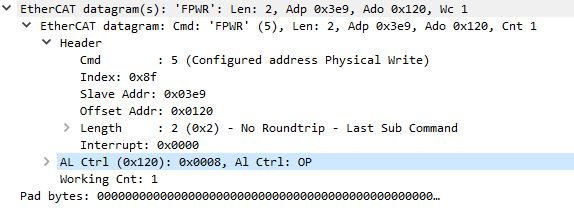
\includegraphics[width=0.7\textwidth]{imgs/result-wireshark-preop-op3.JPG}}}\\
  \subfigure[BRD command to read current AL state register]{\label{subfig:cmd3}{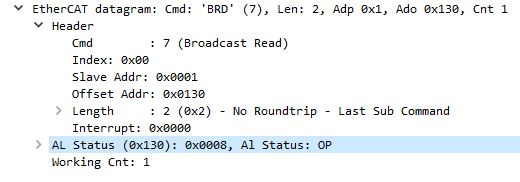
\includegraphics[width=0.7\textwidth]{imgs/result-wireshark-preop-op4.JPG}}}
  \caption{Detailed request and response for a state change. SAFEOP to OP state is the last change starting from INIT state.} %EtherCAT Device Protocol poster from EtherCAT resources
  \label{fig:ecat_wireshark2}
\end{figure}

Finally, in Fig.~\ref{fig:ecat_twincat_objects} the input and outputs part of the object dictionary is shown after it can be 
accessed through TwinCAT3. A whole definition of it is though included in the Appendix~\ref{app:esi_file}.

\begin{figure}[hb]
  \centering
  \subfigure[Process data input]{\label{subfig:objectdictionary1}{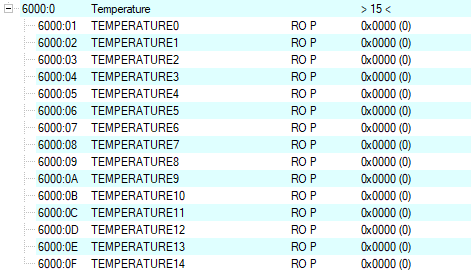
\includegraphics[width=0.68\textwidth]{imgs/result-objectdictionary2.png}}}\\
  \subfigure[Process data output]{\label{subfig:objectdictionary2}{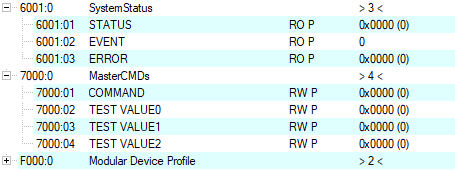
\includegraphics[width=0.68\textwidth]{imgs/result-objectdictionary3.png}}}
  \caption{Object Dictionary from TwinCAT interface.} %EtherCAT Device Protocol poster from EtherCAT resources
  \label{fig:ecat_twincat_objects}
\end{figure} 

% \subsubsection{SPI communication}
% **This is a draft, this might not be needed
% During the final tests some communication errors appeared that were tracked back to the following conditions: %TODO Investigate if this can be called failure modes
% \begin{description}
%     \item[Voltage drops] The on-board Low-Dropout voltage regulator* LDO that provided 3.3 V had random failures, where 
%     the output voltage was from 3.28 to 3.29 V. This caused that the LAN9252 chip was not always ready to work as intended. 
%     This behaviour increased from not-happening to failed completely to start. The mentioned condition obly affected the ESC functionalities,
%     whereas the host MCU worked realiably. To revert this failure mode, an external 3.3V power source was used to continue
%     the current tests. 
%     \item[Noisy channels] While troubleshooting the communication problems mentioned above, an SPI communication
%     test was carried out, such that the effects of different configurations could be characterized. It was concluded that
%     the higher frequencies the SPI was set up, the greater communication faults appeared, leading to error states in the 
%     internal SMs. Moreover, even within rhe stable range, the higher frequencies were not implying shorter execution times.
%     A summary of this observations are presented in the table ~\ref{dummy}.  
% \end{description}
% Regarding the no-improvement of the execution time at a high-speed SPI configuration, the figure ~\ref{dummy} shows 
% a relatevely constant software delay within the words being sent over the SPI bus. Therefore, it does not matter how fast the
% words are sent, for this Software delay is always present *write the order of the delay*. This emergent characteristic of
% the system could be optimized as long as it is determined, whether its impact is critical on the overall throughput of the system.
% The reader should take into consideration the rather small amount of data and the refresh speed of the overall system. However, this
% could be a stating point for improvement of the SOES stack, for those SW delays can be approached by using a fixed sending buffer
% through DMA instead of the usage of the native* API functions that send word by word. A further evaluation of the worthiness*
% of the library changes may be needed.*
% The above mentioned challanges are addressed within the proposals for improvement presented in the section ~\ref{sec:improve}.




